\documentclass[12pt,a4paper,oneside]{article}

% --- Paquetes Básicos ---
\usepackage[utf8]{inputenc}
\usepackage[T1]{fontenc}
\usepackage[spanish,es-tabla]{babel}
\usepackage{lmodern}

% --- Diseño de Página (Márgenes) ---
\usepackage[a4paper,
            top=3cm,
            bottom=3cm,
            left=2.5cm,
            right=2.5cm,
            headheight=15pt,
            footskip=1.5cm]{geometry}

% --- Cabeceras y Pies de Página (Idéntico al original) ---
\usepackage{fancyhdr}
\pagestyle{fancy}
\fancyhf{}
\fancyhead[L]{Memoria Técnica de Adecuación}
\fancyhead[R]{Repostería Barroso Iglesias, SL}
\fancyfoot[C]{\thepage}
\renewcommand{\headrulewidth}{0.4pt}
\renewcommand{\footrulewidth}{0pt}

% --- Gráficos y Tablas ---
\usepackage{graphicx}
\usepackage{booktabs}
\usepackage{array}
\usepackage{caption}
\usepackage{float}


% --- Matemáticas y Símbolos ---
\usepackage{amsmath}
\usepackage{amssymb}

% --- Hipervínculos (Enlaces limpios e interactivos) ---
\usepackage{hyperref}
\hypersetup{
    colorlinks=true,
    linkcolor=black,       
    filecolor=black,
    urlcolor=blue,         % Enlaces en azul estándar para que se identifiquen bien
    citecolor=black,
    pdftitle={Memoria Técnica de Adecuación},
    pdfauthor={Repostería Barroso Iglesias, SL},
}

% --- Ajustes de Párrafos y Espaciado ---
\usepackage{microtype}
\setlength{\parindent}{0pt}
\setlength{\parskip}{1.5ex plus 0.5ex minus 0.2ex}
\renewcommand{\baselinestretch}{1.15}

% --- Inicio del Documento ---
\begin{document}

% Portada
\begin{titlepage}
    \centering
    
    % --- Franja de cabecera ---
    {\large\scshape\textcolor{primarycolor}{Servicio Andaluz de Salud}} \\
    \vspace{0.2cm}
    {\large\bfseries\textcolor{darkcolor}{Hospital Universitario Virgen del Rocío}} \\
    {\small\textcolor{gray}{Hospital de Rehabilitación y Traumatología -- Hospital de San Lázaro}}
    
    \vspace{2.5cm}
    
    % --- Línea Decorativa ---
    \textcolor{primarycolor}{\rule{\linewidth}{1.5mm}}
    \vspace{0.4cm}
    
    % --- Título del Proyecto ---
    {\Huge\bfseries\sffamily\textcolor{primarycolor}{MEMORIA TÉCNICA DE ADECUACIÓN}} \\[0.5cm]
    {\Large\bfseries\sffamily\textcolor{secondarycolor}{Espacios de Cafetería y Puntos de Vending}}
    
    \vspace{0.2cm}
    \textcolor{primarycolor}{\rule{\linewidth}{0.5mm}}
    
    \vspace{2.5cm}
    
    % --- Datos de la Licitación / Expediente ---
    \begin{minipage}{0.8\linewidth}
        \centering
        \textbf{Expediente:} N.º 150/2024 \\
        \textbf{Objeto:} Concesión del Servicio de Cafetería y Manutención de Personal Autorizado.
    \end{minipage}
    
    \vfill
    
    % --- Firmas y Fechas ---
    \begin{minipage}{0.45\linewidth}
        \begin{flushleft} \large
            \emph{Promotor / Adjudicatario:} \\
            \textbf{Repostería Barroso \\ Iglesias, SL}
        \end{flushleft}
    \end{minipage}
    \hfill
    \begin{minipage}{0.45\linewidth}
        \begin{flushright} \large
            \emph{Redactor del Proyecto:} \\
            \textbf{José Ramón Redondo Rosario} \\
            {\small Colegiado N.º 12345}
        \end{flushright}
    \end{minipage}
    
    \vspace{1.5cm}
    
    % --- Fecha ---
    {\large\textcolor{darkcolor}{\today}}
    
\end{titlepage}

\newpage

% Índice general
\pagenumbering{roman}
\tableofcontents
\newpage

\pagenumbering{arabic}

% Secciones del Documento
\section{Introducción y Antecedentes}

\subsection{Agentes del Proyecto}

\subsubsection{Promotor y Adjudicatario del Proyecto}
El promotor de la propuesta de adecuación estética y adjudicatario de la concesión del servicio es la entidad mercantil \textbf{Repostería Barroso Iglesias, SL}, con domicilio social en Sevilla, especialista en gestión de servicios de restauración y alimentación.

\subsubsection{Dirección Técnica y Profesionales Intervinientes}
La redacción de la presente memoria técnica y el diseño de la propuesta de adecuación han sido realizados por el arquitecto y proyectista técnico \textbf{José Ramón Redondo Rosario}, colegiado en Sevilla.

\subsection{Antecedentes y Objeto de la Memoria}
El objeto de esta memoria técnica es definir, justificar y describir detalladamente las actuaciones de remodelación estética, distribución y equipamiento propuestas para la adecuación de los espacios de la cafetería del \textbf{Hospital de Rehabilitación y Traumatología}, perteneciente al \textbf{Hospital Universitario Virgen del Rocío}, de acuerdo con el Pliego de Prescripciones Técnicas (PPT) de la licitación.

El alcance del proyecto contempla exclusivamente la adecuación interior de los comedores (público y de personal) y de la barra de servicio, así como el adecentamiento estético y funcional de la fachada exterior de acceso. Dado que todas las actuaciones son de carácter no estructural (acabados, falsos techos, revestimientos, pintura, iluminación, mobiliario y vegetación), no se altera la volumetría, estructura portante ni la configuración arquitectónica general del edificio.

\subsection{Emplazamiento Objeto de Actuación}
Los espacios objeto de la remodelación se encuentran situados en el complejo hospitalario del Hospital Universitario Virgen del Rocío, concretamente en:
\begin{itemize}
    \item \textbf{Dirección:} Calle Torcuato Luca de Tena s/n, 41013, Sevilla.
    \item \textbf{Edificio:} Hospital de Rehabilitación y Traumatología.
    \item \textbf{Ubicación:} Planta Baja del edificio, con fachada y accesos orientados hacia la vía pública y acera peatonal de la Calle Torcuato Luca de Tena.
\end{itemize}

\subsection{Descripción Geométrica y Superficies Útiles}
La cafetería del Hospital de Rehabilitación y Traumatología cuenta con una superficie útil total de $417,37\text{ m}^2$ y una superficie construida total de $455,43\text{ m}^2$. Los espacios y estancias se adaptan a la geometría preexistente y a los requisitos del servicio sin alterar la distribución estructural de mampostería. En el Cuadro~\ref{tab:superficies} se detalla la relación completa de espacios y sus correspondientes superficies útiles.

\begin{table}[htbp]
    \centering
    \caption{Cuadro de superficies útiles y construidas de la cafetería.}
    \label{tab:superficies}
    \begin{tabular}{lr}
        \toprule
        \textbf{Espacio / Estancia} & \textbf{Superficie Útil ($m^2$)} \\
        \midrule
        Comedor Público & 140,83 \\
        Comedor Personal & 58,28 \\
        Servicio de Barra & 50,03 \\
        Aseo Adaptado & 5,48 \\
        Vestíbulo Aseos & 2,70 \\
        Aseo Masculino & 3,61 \\
        Aseo Femenino & 3,61 \\
        Vestíbulo & 22,47 \\
        Espacio sin Uso & 9,00 \\
        Propano & 2,85 \\
        Climatización & 12,85 \\
        Sala de Lavado & 21,54 \\
        Cocina & 27,10 \\
        Preparaciones & 14,65 \\
        Pasillo Cámaras & 15,00 \\
        Almacén & 7,12 \\
        Cámaras & 14,52 \\
        Cuarto Basuras & 2,49 \\
        Otros (N/A) & 3,24 \\
        \midrule
        \textbf{Superficie Útil Total} & \textbf{417,37} \\
        \textbf{Superficie Construida} & \textbf{455,43} \\
        \bottomrule
    \end{tabular}
\end{table}

\newpage

\section{Descripción del Servicio y Organización}
\label{sec:descripcion}

\subsection{Servicios de Cafetería}
Se establecen dos modalidades de servicio de cafetería diferenciadas para atender de manera óptima las necesidades de cada colectivo:

\subsubsection{Cafetería de Público}
Destinada a visitantes, familiares y pacientes ambulatorios. Ofrecerá una amplia gama de productos saludables, menús diarios y opciones especiales (sin gluten, vegetarianas, etc.).

\subsubsection{Cafetería de Profesionales}
Destinada al personal del centro hospitalario. Contará con tarifas bonificadas según pliegos y un sistema de servicio ágil para adaptarse a los tiempos de descanso del personal sanitario.

\subsection{Servicio de Manutención para Personal Autorizado}
El servicio de manutención está especialmente diseñado para el personal de guardia médica u otros profesionales autorizados del \textbf{Hospital de Rehabilitación y Traumatología}. 
\begin{itemize}
    \item \textbf{Desayuno y Cafés:} Dispensación en horarios establecidos directamente en las áreas habilitadas.
    \item \textbf{Almuerzo y Cena:} Menús equilibrados nutricionalmente, supervisados por el servicio de dietética del hospital.
    \item \textbf{Distribución en Unidades:} Protocolo de entrega de comidas en bandejas térmicas para el personal que no pueda abandonar su puesto de guardia.
\end{itemize}

\subsection{Plan de Control de Higiene y Alérgenos}
Toda la manipulación de alimentos se regirá bajo un estricto sistema de \textbf{Análisis de Peligros y Puntos de Control Crítico (APPCC)}, garantizando la trazabilidad y seguridad alimentaria en todo momento. Se prestará especial atención a la identificación de alérgenos según el Reglamento (UE) N.º 1169/2011 \cite{reglamento_alergenos}.

\newpage

\section{Propuesta de Adecuación y Equipamiento}
\label{sec:adecuacion}

\subsection{Obras y Reformas Propuestas}
Para optimizar el flujo de usuarios y mejorar el confort térmico y acústico de las cafeterías, se proponen las siguientes actuaciones de adecuación física:
\begin{enumerate}
    \item Renovación de revestimientos y pavimentos con materiales antideslizantes y de fácil limpieza.
    \item Mejora del sistema de climatización y ventilación.
    \item Rediseño de la línea de self-service para agilizar los tiempos de espera en las horas punta.
\end{enumerate}

\subsection{Equipamiento y Mobiliario}
Se renovará la maquinaria de cocina y barra, priorizando equipos de alta eficiencia energética para reducir la huella de carbono del centro hospitalario. En la Tabla~\ref{tab:equipos} se resume el equipamiento principal a incorporar.

\begin{table}[htbp]
    \centering
    \caption{Relación de equipamiento principal propuesto.}
    \label{tab:equipos}
    \begin{tabular}{llcc}
        \toprule
        \textbf{Descripción} & \textbf{Ubicación} & \textbf{Unidades} & \textbf{Clase Energética} \\
        \midrule
        Lavavajillas de cúpula industrial & Cocina Principal & 2 & A+++ \\
        Vitrina expositora refrigerada & Barra Cafetería & 3 & A+ \\
        Cafetera exprés profesional & Barra Cafetería & 2 & A \\
        Hornos de convección mixtos & Cocina Principal & 1 & A++ \\
        \bottomrule
    \end{tabular}
\end{table}

\subsection{Puntos de Venta Automática (Vending)}
Los puntos de vending serán renovados por máquinas inteligentes (smart vending) con lector de tarjetas bancarias, dispositivos móviles y tarjetas de empleado del HUVR. Al menos el $30\%$ de los productos ofrecidos corresponderán a la gama de alimentación saludable (fruta fresca, frutos secos naturales, lácteos desnatados, bebidas sin azúcares añadidos), cumpliendo las directrices de la Consejería de Salud y Consumo \cite{salud_andalucia}.

\newpage

% --- SECCIÓN 4: CATÁLOGO DE MATERIALES ---
\section{Propuesta Técnica de Acabados Estéticos (Catálogo de Materiales)}
\label{sec:catalogo}
A continuación se detallan las fichas técnicas y características físicas del catálogo de materiales y mobiliario seleccionados para la adecuación de la cafetería del Hospital de Rehabilitación y Traumatología, asegurando la homogeneidad y cumplimiento de las directrices sanitarias.

\subsection{Revestimientos de Suelo (Solados)}
\label{sec:cat_6_1}
\subsection{Pavimento Continuo de Resina de Poliuretano (Sin juntas)}
\label{solado:resina}
\textbf{Descripción:} Sistema de pavimento continuo elástico de resina de poliuretano, tipo Tecnofloor PU-3010del fabricante español Tecnopol. Aplicado en estado líquido y autonivelante para formar una superficie monolítica de 2 a 3 mm de espesor, completamente estanca, higiénica y sin juntas de unión. Seleccionado en color beige arena (RAL 1015) de aspecto similar a la muestra de imagen con acabado mate satinado antideslizante. Ofrece absorción acústica de ruidos de impacto, confort al caminar, resistencia química a desinfectantes hospitalarios y fácil limpieza diaria. Ficha de producto disponible en el \href{https://www.aplikamolina.com/suelo-resina-epoxi-clinicas.html#prettyPhoto}{Sitio Web}.

\textbf{Uso en la memoria:} Suelo continuo del comedor de personal, comedor de público y barra de servicio (Ap. 2.1 y 2.2).

\begin{figure}[H]
    \centering
    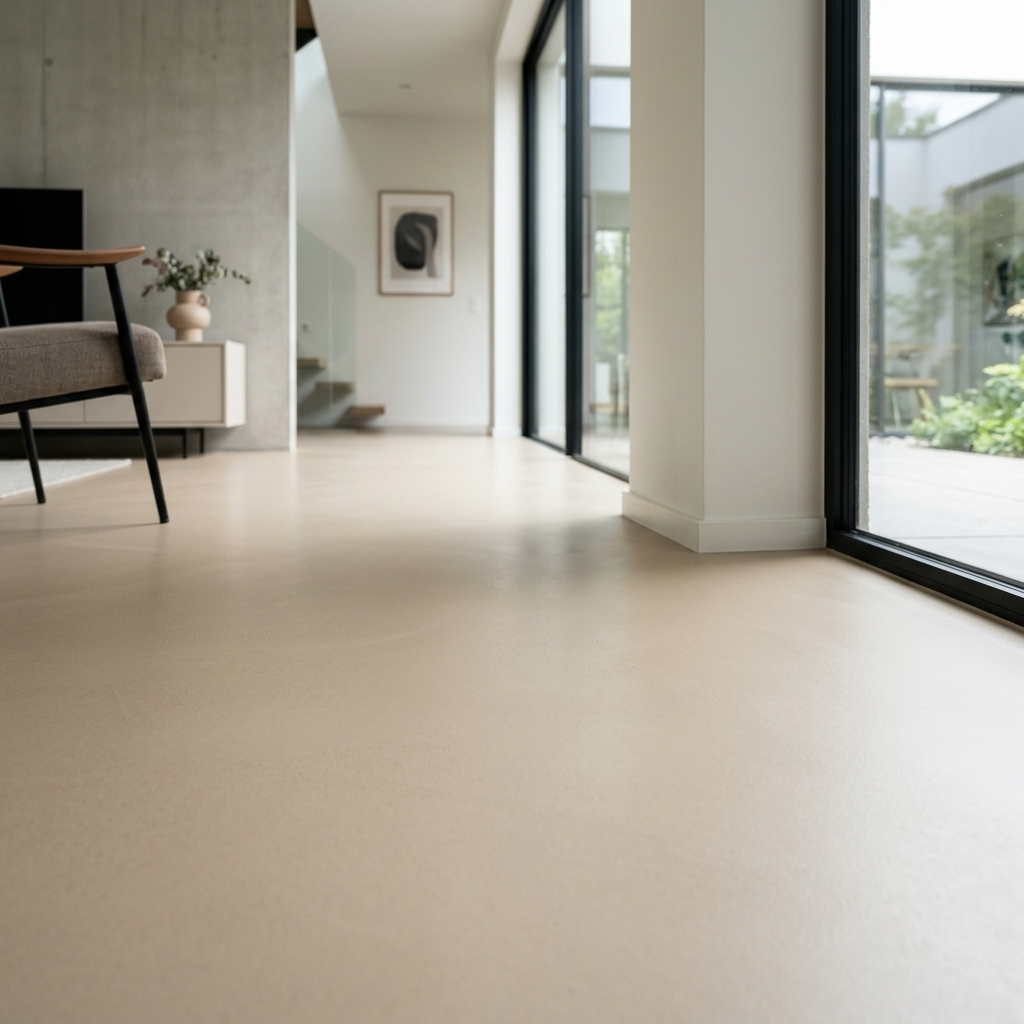
\includegraphics[width=0.7\linewidth]{images/figura_1.png}
    \caption{Pavimento continuo de poliuretano}
    \label{fig:resina}
\end{figure}


\subsection{Canto Rodado Decorativo Crema/Blanco}
\label{solado:canto}
\textbf{Descripción:} Piedra triturada y redondeada de mármol natural en tamaño de granulometría de 12-18 mm. Presenta un tono crema claro y textura suave, excelente para cobertura estética en jardinería, facilitando la filtración de agua y reduciendo la evaporación del sustrato. Suministrado por distribuidores locales y viveros de Sevilla. Ficha de producto disponible en el \href{https://www.obramat.es/productos/grava-blanca-12-18-mm-20-kg-25036734.html}{Sitio Web de Obramat}.

\textbf{Uso en la memoria:} Cobertura ornamental y drenaje en las jardineras de exterior (Ap. 3.4).

\begin{figure}[H]
    \centering
    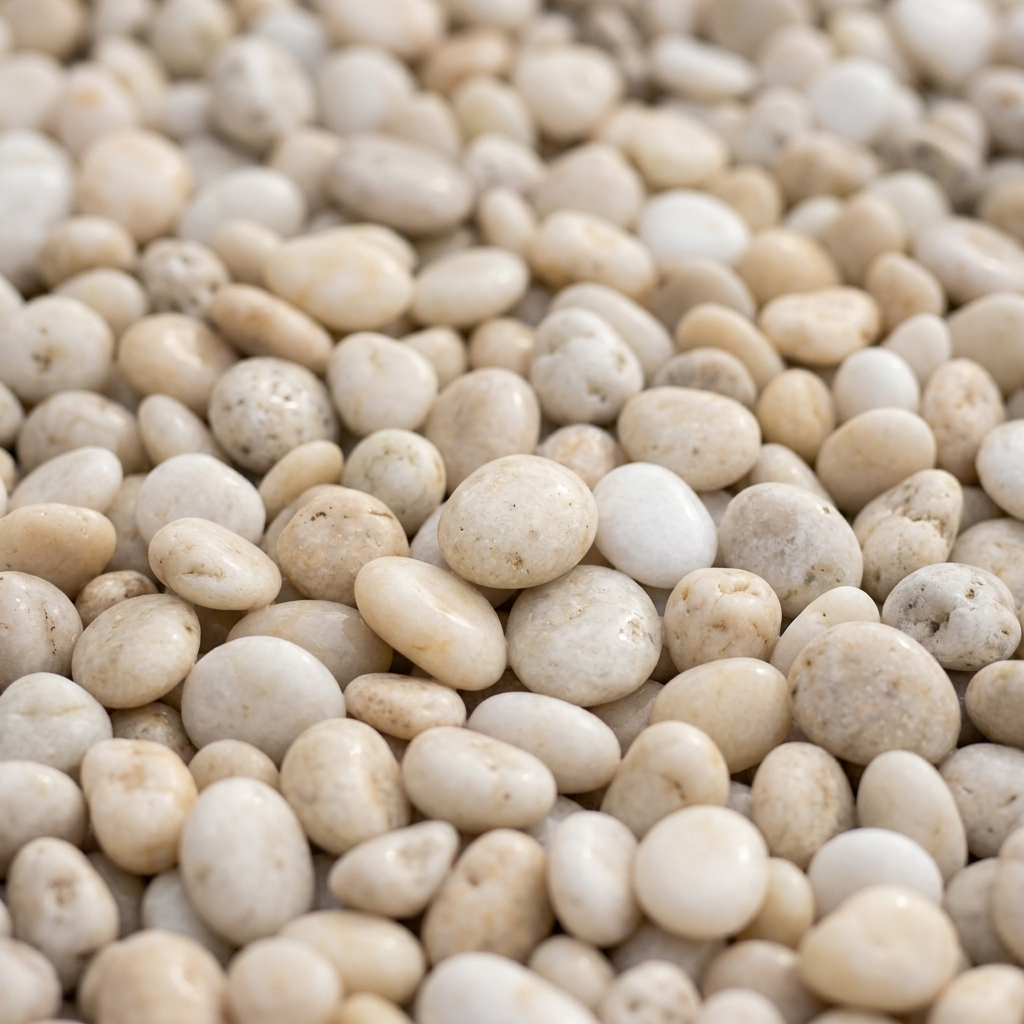
\includegraphics[width=0.7\linewidth]{images/figura_3.png}
    \caption{Canto rodado de mármol crema decorativo}
    \label{fig:canto}
\end{figure}


\subsection{Mobiliario y Equipamiento de Comedores}
\label{sec:cat_6_2}
\subsection{Mesa Rectangular Resol DESSA (160x90 cm)}
\label{mob:mesa_rect}
\textbf{Descripción:} Diseñada por Josep Lluscá. Mesa rectangular de comedor con estructura interior de acero zincado pintado por pulverización en color blanco y sobre y patas inyectadas en polipropileno copolímero de alta resistencia, con tratamiento anti-UV para evitar la decoloración. Dimensiones: 160 cm de largo, 90 cm de ancho y 74 cm de altura. Peso neto: 16.75 kg. Certificaciones de resistencia para uso público intenso (UNE-EN 15372). Ficha de producto disponible en el \href{https://www.makro.es/marketplace/product/903d3d04-0dd5-4579-93cb-b7091788f8ad}{Sitio Web de Makro}.

\textbf{Uso en la memoria:} Mesas de comedor de personal (1 ud.) y comedor de público (8 uds.) (Ap. 2.1 y 2.2).

\begin{figure}[H]
    \centering
    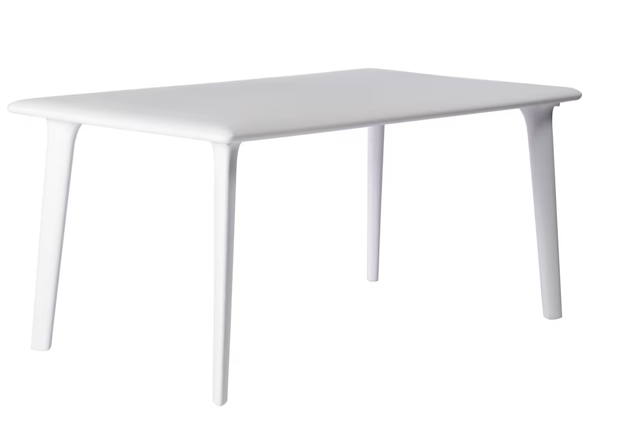
\includegraphics[width=0.7\linewidth]{images/figura_4.png}
    \caption{Mesa rectangular Resol Dessa}
    \label{fig:mesa_rect}
\end{figure}


\subsection{Silla Confidente Actiu Noom (Serie 50 - Base Patín)}
\label{mob:silla_conf}
\textbf{Descripción:} Diseñada por Alegre Design. Silla confidente ligera y ergonómica sin brazos, de respaldo alto. Estructura de base patín fabricada en tubo cilíndrico de acero laminado en caliente de 13 mm de diámetro y 2 mm de espesor, con recubrimiento de pintura epoxi de 90 micras de espesor en color blanco mate. Carcasa inyectada de polipropileno (P.P.) de 5 mm de espesor reforzado con fibra de vidrio, con acabado texturado antideslizante. Conteras de polipropileno con fieltro antideslizante integrado. Dimensiones totales: Altura de 836 mm, anchura de 522 mm y profundidad de 543 mm. Dimensiones del asiento: Altura de 473 mm, anchura de 443 mm y profundidad de 519 mm. Certificada para uso intensivo en oficinas y colectividades (UNE-EN 16139). Ficha de producto disponible en el \href{https://spacio.es/producto/sillas/sillas-confidente/sillas-para-hogar/silla-confidente-base-patin-actiu-noom-serie-50/?srsltid=AfmBOoro-D21eeNqrwztycS8rSaA7fgDVHFSJ8n9pnpir-qXSPCX6CfS}{Sitio Web de Spacio}.

\textbf{Uso en la memoria:} Sillas bajas de comedor de personal (36 uds.) y comedor de público (42 uds.) (Ap. 2.1 y 2.2).

\begin{figure}[H]
    \centering
    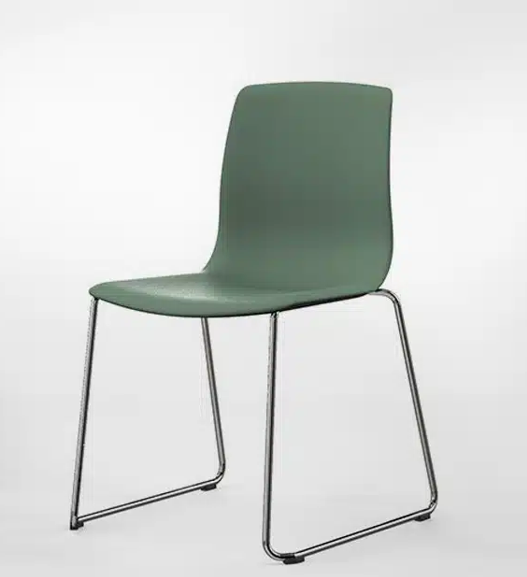
\includegraphics[width=0.7\linewidth]{images/figura_5.png}
    \caption{Silla confidente Actiu Noom Serie 50}
    \label{fig:silla_conf}
\end{figure}


\subsection{Mesa Cuadrada Resol DESSA (90x90 cm)}
\label{mob:mesa_cuad}
\textbf{Descripción:} Diseñada por Josep Lluscá. Mesa cuadrada de comedor exterior con estructura interior de acero zincado y sobre y patas inyectadas en polipropileno de alta densidad en color blanco, con tratamiento anti-UV. Dimensiones: 90 cm de largo, 90 cm de ancho y 74 cm de altura. Peso neto: 12.5 kg. Certificaciones de resistencia para uso público exterior (UNE-EN 581). Ficha de producto disponible en el \href{https://www.makro.es/marketplace/product/3b3239d9-ee56-46d0-be31-6512a1e75539}{Sitio Web de Makro}.

\textbf{Uso en la memoria:} Mesas del comedor de público (5 uds.) (Ap. 2.2).

\begin{figure}[H]
    \centering
    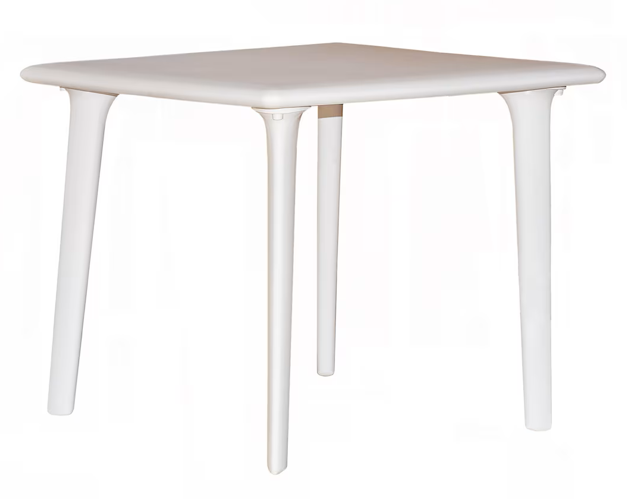
\includegraphics[width=0.7\linewidth]{images/figura_6.png}
    \caption{Mesa cuadrada Resol Dessa}
    \label{fig:mesa_cuad}
\end{figure}


\subsection{Mesa Baja Alargada Kube de Ofiprix (240x142 cm)}
\label{mob:mesa_kube}
\textbf{Descripción:} Mesa de reuniones doble con encimera continua en acabado de melamina blanca mate de 30 mm de espesor y cantos de PVC. Estructura de acero con patas retranqueadas pintadas por pulverización epoxi en color blanco mate, facilitando la comodidad de los usuarios. Equipada con una bandeja pasacables electrificable y tapas pasacables de 80 mm en superficie para una gestión óptima de la conectividad. Dimensiones: 240 cm de largo, 142 cm de ancho y 74 cm de alto. Ficha de producto disponible en el \href{https://www.ofiprix.com/es/mesa-de-reuniones-doble-kube-encimera-continua-fondo-142-cm-estructura-blanca?combination=186813&gad_source=1&gad_campaignid=16129922352&gbraid=0AAAAAD8J8PG2ocXTygTljI1icJwMTQgyQ&gclid=EAIaIQobChMImZ6Jm-T-lAMViNhEBx3ZVCOBEAkYAyABEgI_O_D_BwE#/228-colorvalid-blanco_mate/708-medida-240x142}{Sitio Web de Ofiprix}.

\textbf{Uso en la memoria:} Mesas bajas largas para el comedor de personal (4 uds.) (Ap. 2.1).

\begin{figure}[H]
    \centering
    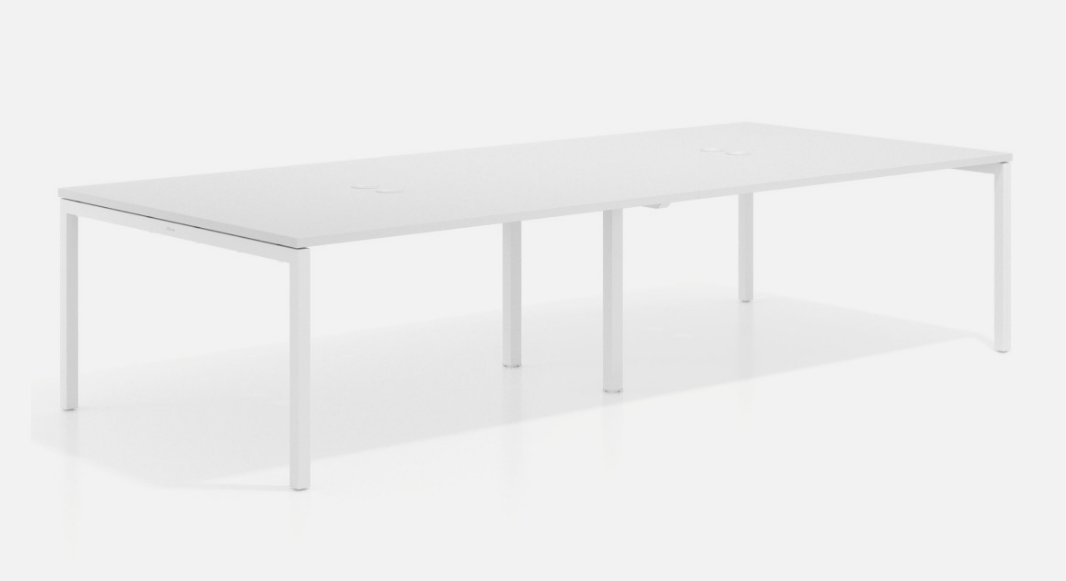
\includegraphics[width=0.7\linewidth]{images/figura_8.png}
    \caption{Mesa reuniones Ofiprix}
    \label{fig:mesa_kube}
\end{figure}


\subsection{Taburete Alto de Jardín Brenza (SKLUM)}
\label{mob:taburete}
\textbf{Descripción:} Taburete alto de diseño contemporáneo y estilo escandinavo, apto para interior y exterior. Fabricado en una sola pieza monobloque de polipropileno inyectado con acabado mate y protección contra radiación solar UV. Cuenta con respaldo bajo curvado ergonómico, reposapiés integrado en su estructura y tacos protectores antideslizantes. Dimensiones: 93 cm de altura, 51 cm de anchura y 51 cm de profundidad. Peso: 4.90 kg. Ficha de producto disponible en el \href{https://www.sklum.com/es/comprar-packs-de-taburetes-de-jardin/227241-pack-de-4-taburetes-altos-de-jardin-apilables-en-polipropileno-brenza.html?id_c=673316}{Sitio Web de SKLUM}.

\textbf{Uso en la memoria:} Taburetes altos en la zona de barra y comedor de público (10 uds.) (Ap. 2.2).

\begin{figure}[H]
    \centering
    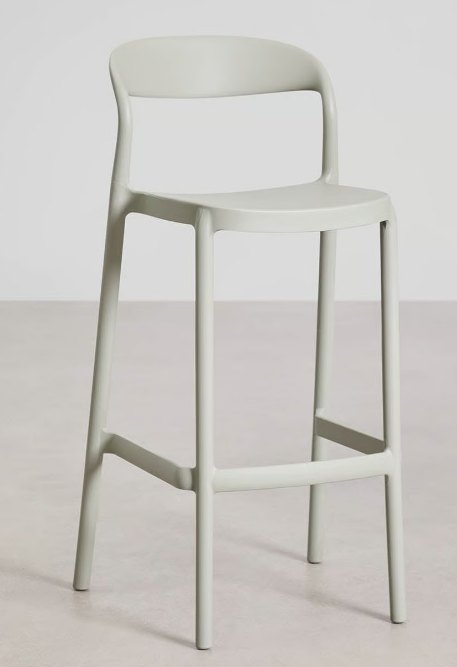
\includegraphics[width=0.7\linewidth]{images/figura_10.png}
    \caption{Taburete alto Sklum}
    \label{fig:taburete}
\end{figure}


\subsection{Mesa Alta de Bar (Makro)}
\label{mob:mesa_alta}
\textbf{Descripción:} Mesa alta redonda de bistró y recepción. Estructura de pie central cilíndrico de acero lacado o aluminio con base de disco circular ponderada que garantiza gran estabilidad al conjunto. Tablero redondo superior de melamina o tablero compacto en color blanco mate, apto para la limpieza frecuente con desinfectantes de uso público. Dimensiones: Altura de 110 cm y diámetro de 60 cm. Ficha de producto disponible en el \href{https://www.makro.es/marketplace/product/3bf850cf-f497-4128-93cd-c8676b2957d7}{Sitio Web de Makro}.

\textbf{Uso en la memoria:} Mesas altas de apoyo en el comedor de público (Ap. 2.2).

\begin{figure}[H]
    \centering
    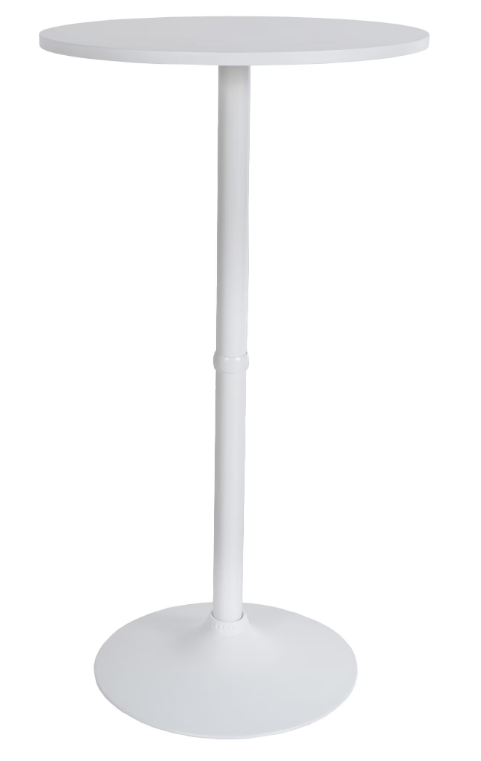
\includegraphics[width=0.7\linewidth]{images/figura_11.png}
    \caption{Mesa alta de bar Makro}
    \label{fig:mesa_alta}
\end{figure}


\subsection{Luminarias e Iluminación Decorativa}
\label{sec:cat_6_3}
\subsection{Iluminación General Empotrada - Downlight LED (Arkoslight Swap M)}
\label{lum:downlight}
\textbf{Descripción:} Foco empotrado circular de diseño minimalista. Diámetro de corte de 75 mm y bisel extrafino lacado en blanco mate. Potencia de 7W, alimentación a 24V DC, flujo luminoso nominal de 910 lm, temperatura de color blanco cálido de 3000K y un índice de reproducción cromática excelente (CRI ¿90) para una visualización natural de los alimentos. ´Optica de reflector de policarbonato metalizado con ángulo de apertura de 36º(flood), equipado con difusor opal antideslumbrante para un confort visual UGR ¡19. Vida útil L80B10 de 60.000 horas y grado de protección IP20 (IP54 en la cara expuesta). Ficha de producto disponible en el \href{https://www.arkoslight.com/es/producto/swap-m/}{Sitio Web} de Arkoslight.

\textbf{Uso en la memoria:} Iluminación general empotrada en el falso techo de toda la cafetería interior (Ap. 2.3).

\begin{figure}[H]
    \centering
    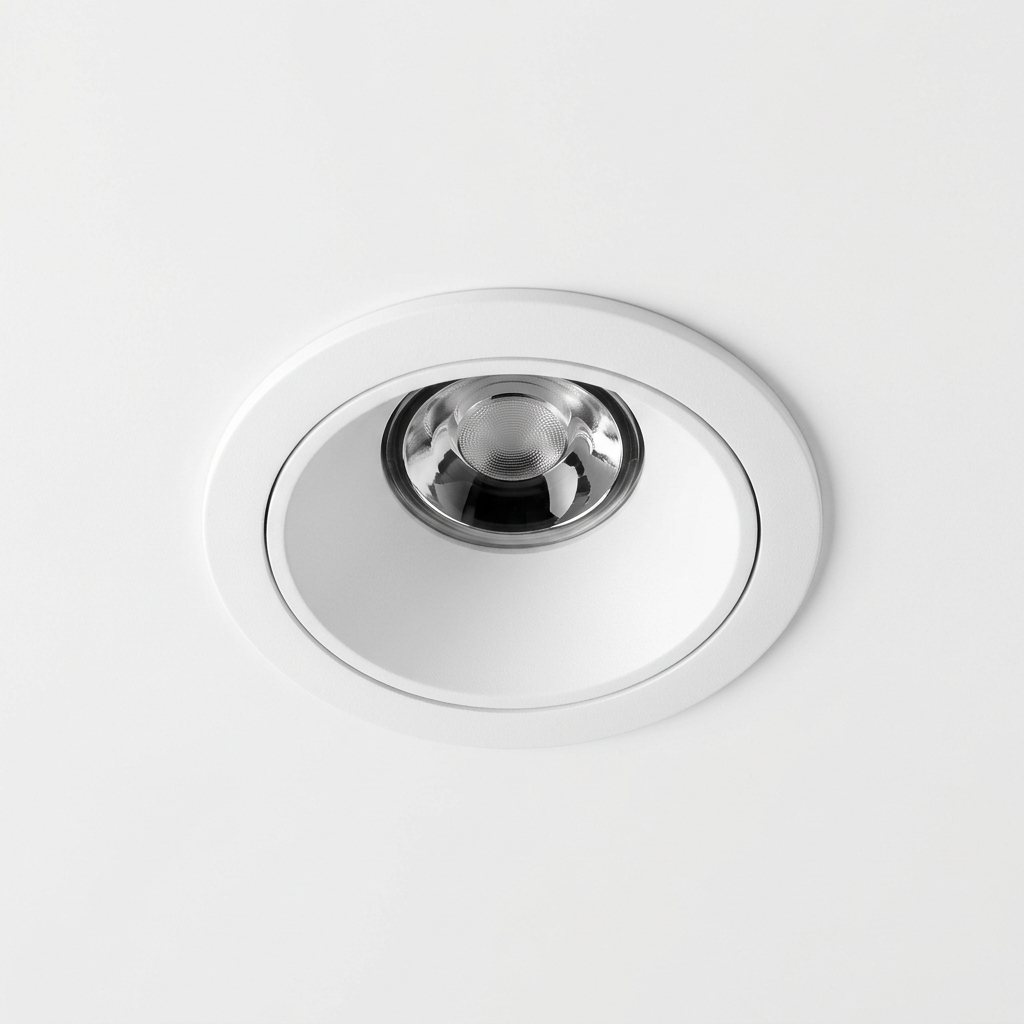
\includegraphics[width=0.7\linewidth]{images/figura_12.png}
    \caption{Foco empotrado Downlight LED Arkoslight Swap M}
    \label{fig:downlight}
\end{figure}


\subsection{Aplique LED Cilíndrico Exterior (Faro Barcelona Cylinder)}
\label{lum:aplique_cyl}
\textbf{Descripción:} Aplique de pared estanco para exteriores con diseño cilíndrico vertical y emisión de luz descendente (o bidireccional). Fabricado en aluminio inyectado de alta pureza con acabado en color negro mate. Difusores de cristal templado transparente sellados con juntas de silicona para garantizar una estanqueidad IP65 y resistencia a impactos IK08. Equipado con un módulo LED COB de 8W (o dos de 6W), flujo luminoso de 650 lm y temperatura de color de 3000K (luz cálida). Dimensiones: 150 mm de altura, 80 mm de diámetro. Ficha de producto disponible en el \href{https://faro.es/es/producto/stan-aplique-negro/}{Sitio Web de Faro Barcelona}.

\textbf{Uso en la memoria:} Iluminación decorativa y funcional en la fachada exterior (Ap. 3.3).

\begin{figure}[H]
    \centering
    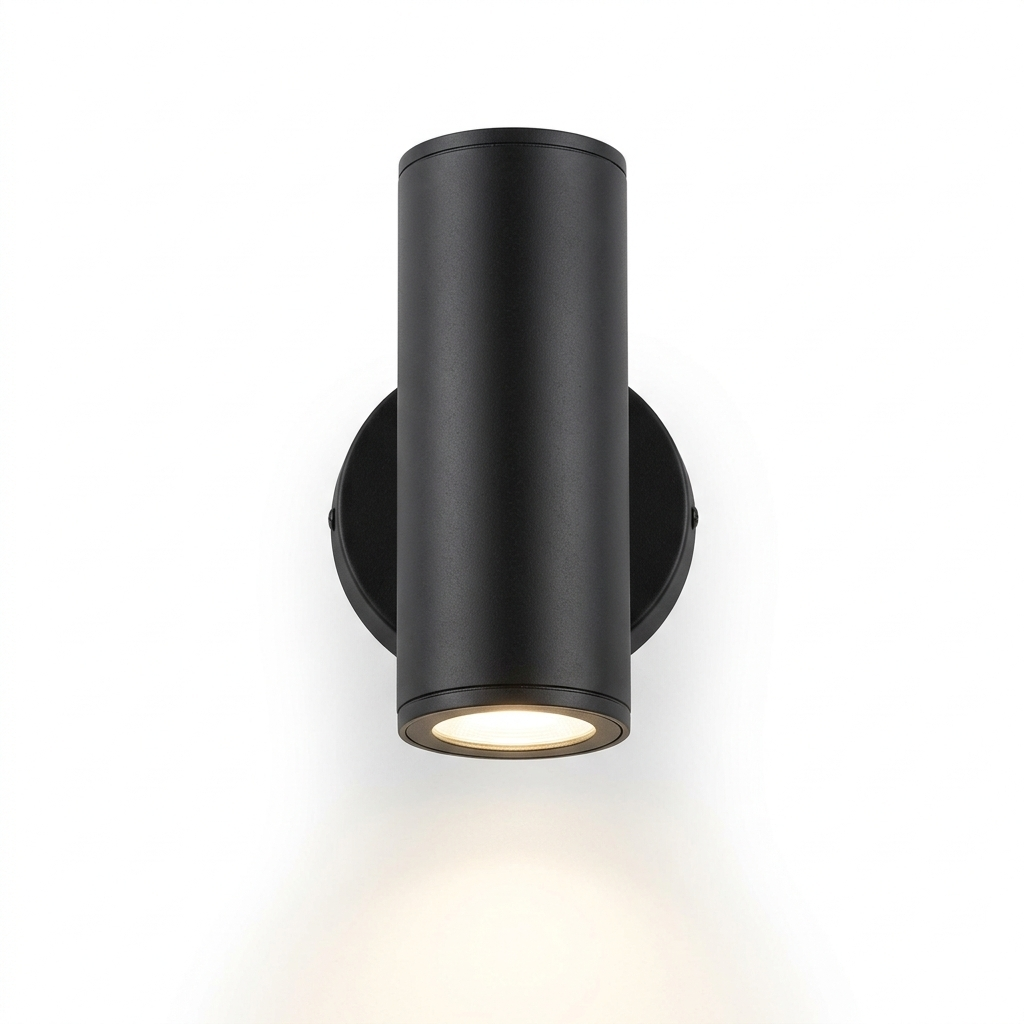
\includegraphics[width=0.7\linewidth]{images/figura_13.png}
    \caption{Aplique cilíndrico exterior Faro Barcelona Cylinder}
    \label{fig:aplique_cyl}
\end{figure}


\subsection{Luminaria Suspendida de Barra - Globo de Vidrio (Faro Barcelona Pam)}
\label{lum:lampara_pam}
\textbf{Descripción:} Lámpara colgante decorativa con difusor esférico en forma de globo de vidrio soplado transparente (diámetro de 250 mm) y portalámparas cilíndrico metálico con acabado en color blanco o cromo. Suspensión mediante cable eléctrico ajustable en altura hasta 150 cm. Equipada con casquillo E27 para bombilla decorativa de filamento LED de 8W, flujo de 720 lm y temperatura de color blanco cálido de 2700K (luz muy cálida), aportando una atmósfera acogedora y transparente. Ficha de producto disponible en el Sitio Web de Iluminación Coben.

\textbf{Uso en la memoria:} Iluminación de acento suspendida sobre la barra de servicio (8 uds.) (Ap. 2.2).

\begin{figure}[H]
    \centering
    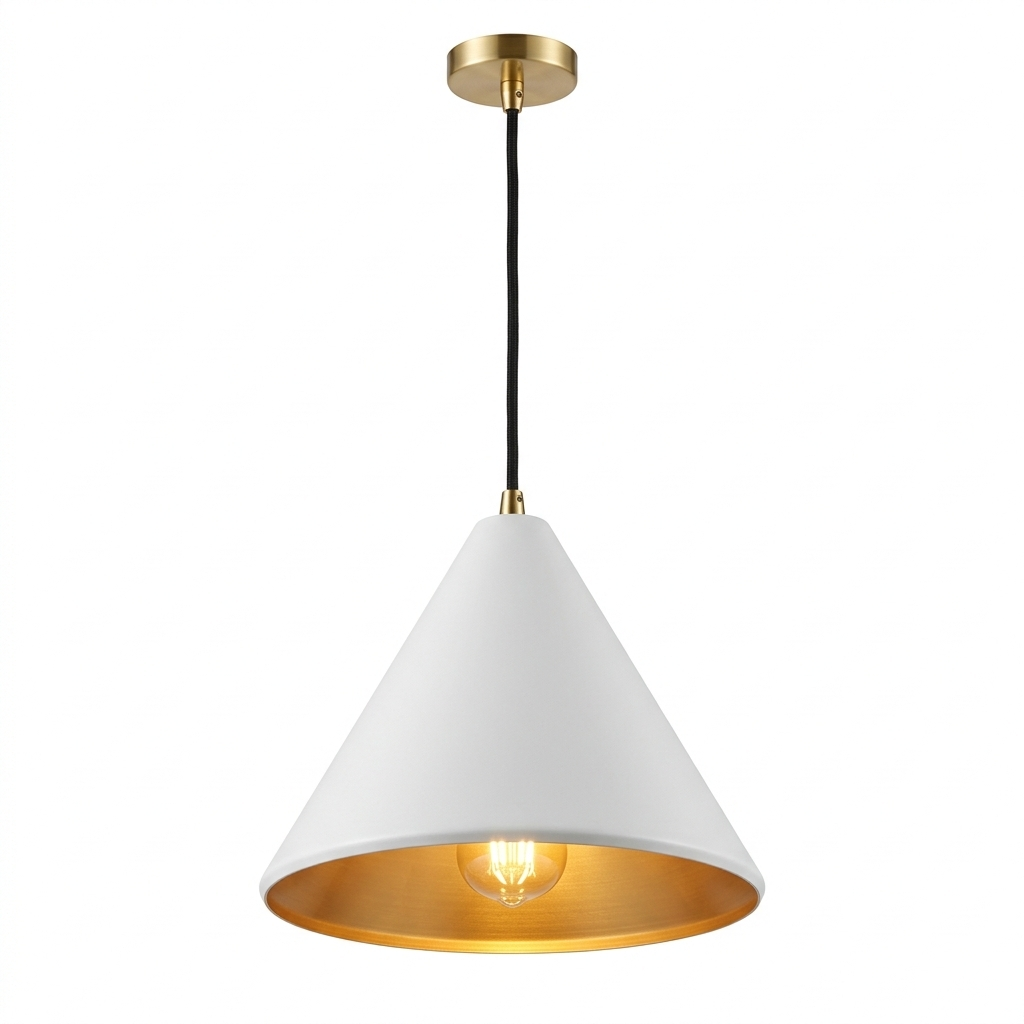
\includegraphics[width=0.7\linewidth]{images/figura_15.png}
    \caption{Lámpara colgante de globo de vidrio Faro Barcelona Pam}
    \label{fig:lampara_pam}
\end{figure}


\subsection{Tira de LED de Acentuación (Prilux Flexiled IP20)}
\label{lum:tira_led}
\textbf{Descripción:} Tira de LED flexible continua de alta densidad (120 LEDs por metro) para evitar el efecto de sombreado o puntos de luz marcados. Tensión de funcionamiento 24V DC, consumo de 9.6 W/m, flujo luminoso de 960 lm/m y temperatura de color de 3000K con CRI ¿90. Instalada en el interior de un perfil de aluminio anodizado extrusionado disipador de calor y cerrada con difusor de policarbonato opalizado curvo para una distribución de luz indirecta homogénea. Ficha de producto disponible en el \href{https://www.prilux.com/es/productos/flexiled/}{Sitio Web de Prilux}.

\textbf{Uso en la memoria:} Iluminación indirecta bajo la barra de servicio y en el foseado del techo interior y exterior (Ap. 2.2 y 3.3).

\begin{figure}[H]
    \centering
    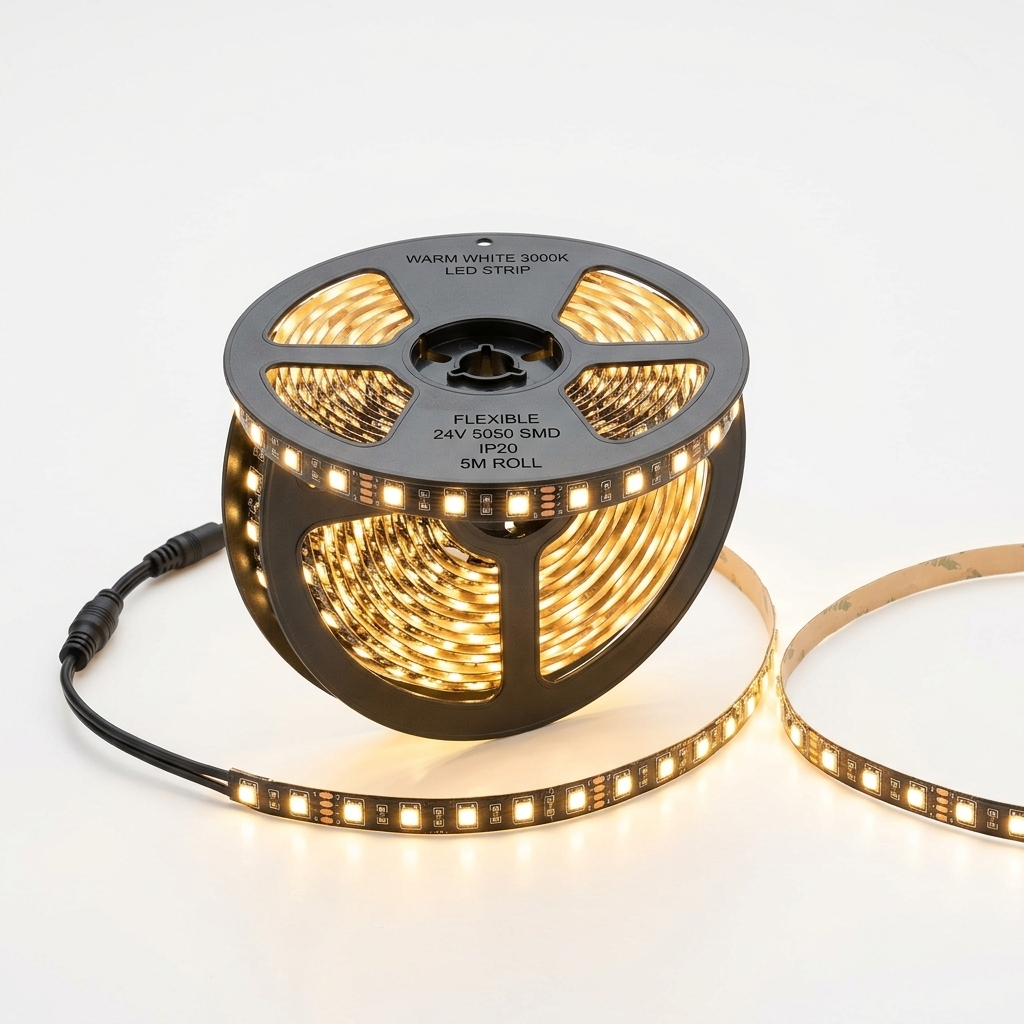
\includegraphics[width=0.7\linewidth]{images/figura_16.png}
    \caption{Tira de LED flexible Prilux Flexiled}
    \label{fig:tira_led}
\end{figure}


\subsection{Aplique Vertical de Pared Exterior (Faro Barcelona Amen)}
\label{lum:aplique_amen}
\textbf{Descripción:} Aplique de pared estanco para exteriores con diseño vertical estilizado. Estructura de aluminio inyectado acabado en color negro o gris oscuro mate y difusor esférico de vidrio soplado opalizado que proporciona una distribución de luz difusa, uniforme y sin deslumbramientos. Grado de protección IP65 y resistencia a impactos IK07. Equipado con portalámparas E27 para bombilla LED de 6W, flujo luminoso de 540 lm y temperatura de color de 3000K (luz cálida). Dimensiones: 250 mm de altura total. Ficha de producto disponible en el \href{https://faro.es/es/iluminacion/apliques/}{Sitio Web de Faro Barcelona}.

\textbf{Uso en la memoria:} Aplique vertical en las columnas del exterior de la fachada (Ap. 3.3).

\begin{figure}[H]
    \centering
    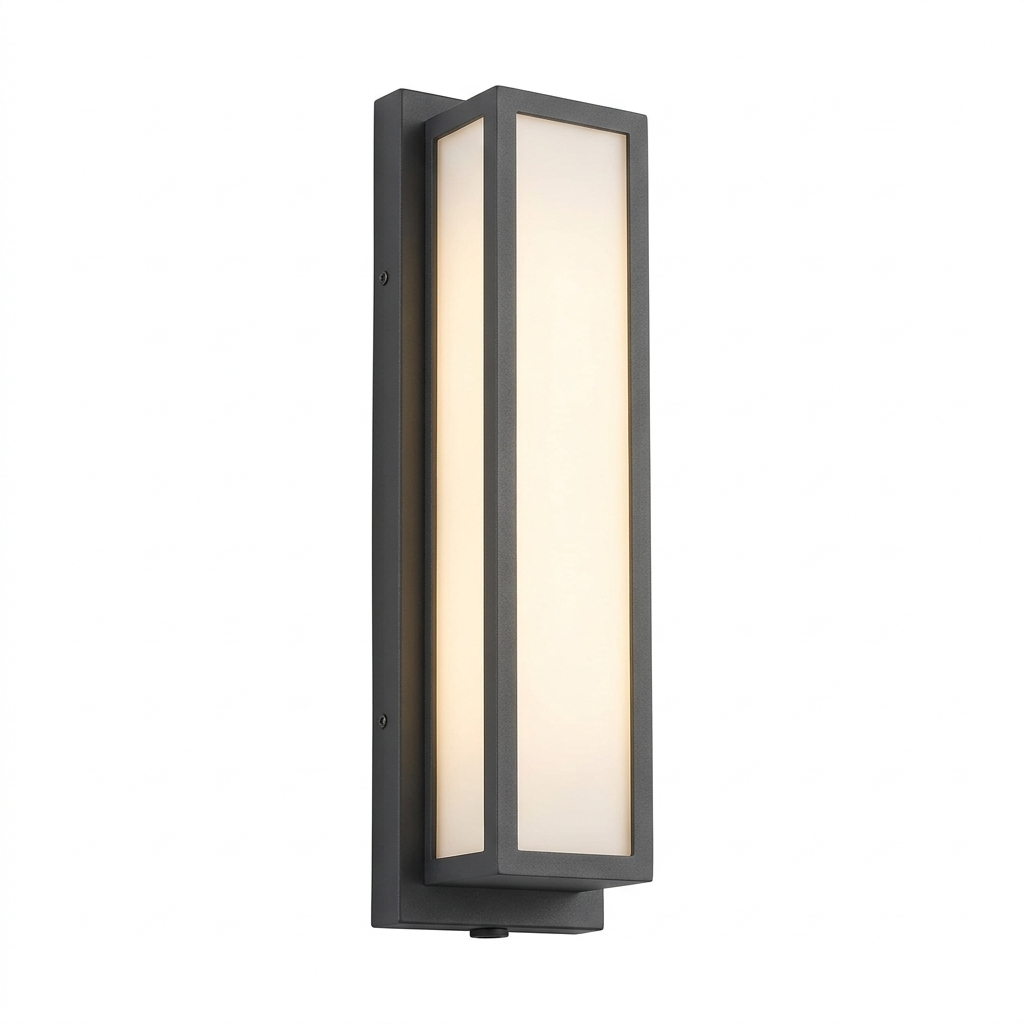
\includegraphics[width=0.7\linewidth]{images/figura_17.png}
    \caption{Aplique vertical exterior Faro Barcelona Amen}
    \label{fig:aplique_amen}
\end{figure}


\subsection{Proyector LED de Acentuación con Piqueta (Faro Barcelona Spike)}
\label{lum:proyector}
\textbf{Descripción:} Foco proyector estanco para exterior con estaca/piqueta de anclaje para hincar en tierra. Cuerpo fabricado en aluminio inyectado de alta pureza con acabado en color negro y difusor de vidrio transparente templado. Grado de protección IP65 y resistencia al impacto IK08. Equipado con módulo LED de 3W o 6W de potencia, luz cálida (3000K) y ángulo de apertura concentrado de 25ºa 40º, ideal para realce lumínico vertical de plantas. Alimentación a 220-240V AC. Ficha de producto disponible en el \href{https://faro.es/es/producto/seth-proyector-negro/}{Sitio Web de Faro Barcelona}.

\textbf{Uso en la memoria:} Proyectores de acentuación integrados en los maceteros exteriores (Ap. 3.3).

\begin{figure}[H]
    \centering
    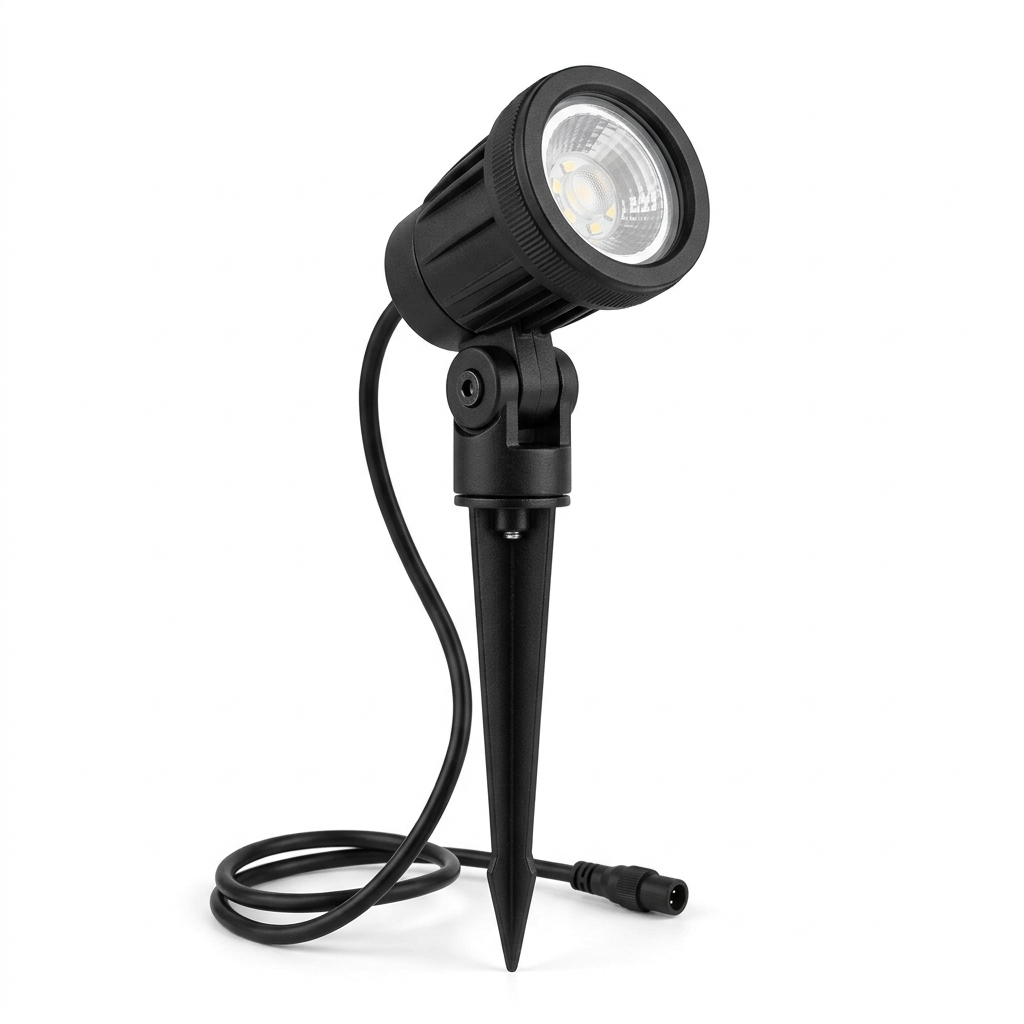
\includegraphics[width=0.7\linewidth]{images/figura_18.png}
    \caption{Proyector LED de jardín con piqueta Faro Barcelona Spike/Seth}
    \label{fig:proyector}
\end{figure}


\subsection{Luminaria de Suspensión de Plato (Faro Barcelona - Mute Verde)}
\label{lum:lampara_mute}
\textbf{Descripción:} Lámpara de suspensión de diseño escandinavo con pantalla en forma de plato hondo fabricada en fieltro de PET reciclado con propiedades de absorción acústica, acabado en color verde oliva/salvia. Diámetro de 60 cm y altura de 25 cm. Suspendida por cable textil ajustable en altura. Equipado con placa LED integrada de 16W de potencia, luz cálida de 3000K y flujo luminoso de 1500 lm. Idónea para mesas altas en cafeterías de alto tránsito. Ficha de producto disponible en el \href{https://www.iluminacioncoben.com/productos/colgante-mute-de-faro/}{Sitio Web de Iluminación Coben}.

\textbf{Uso en la memoria:} Luminarias acústicas suspendidas en los techos del comedor de público (7 uds.) (Ap. 2.3).

\begin{figure}[H]
    \centering
    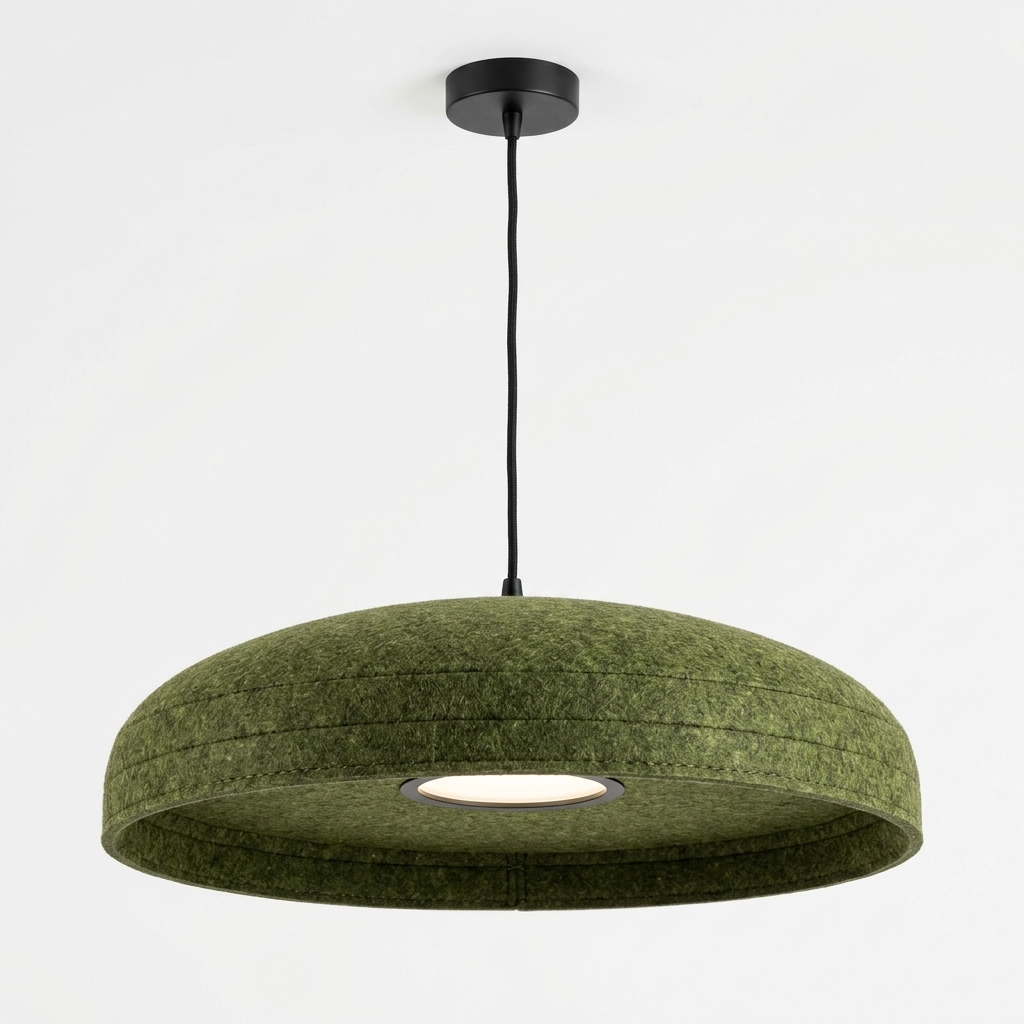
\includegraphics[width=0.7\linewidth]{images/figura_19.png}
    \caption{Lámpara acústica de suspensión Faro Barcelona Mute}
    \label{fig:lampara_mute}
\end{figure}


\subsection{Revestimientos y Decoración de Paredes}
\label{sec:cat_6_4}
\subsection{Aplacado de Piedra Natural (Exterior)}
\label{wall:aplacado}
\textbf{Descripción:} Placas de piedra caliza natural tipoCaliza Crema de Antequera(canteras de Málaga, distribución local en Sevilla a través deMármoles Sevillau otros talleres de cantería). Formato de 60×30 cm, espesor 2 cm, acabado abujardado o arenado para exteriores, colocado mediante adhesivo cementoso flexible C2TE y anclajes mecánicos de acero inoxidable de seguridad. Ficha de producto disponible en el \href{https://www.marmolessevilla.com/}{Sitio Web de Mármoles Sevilla}.

\textbf{Uso en la memoria:} Revestimiento de piedra caliza natural en paramentos exteriores de fachada (Ap. 3.1).

\begin{figure}[H]
    \centering
    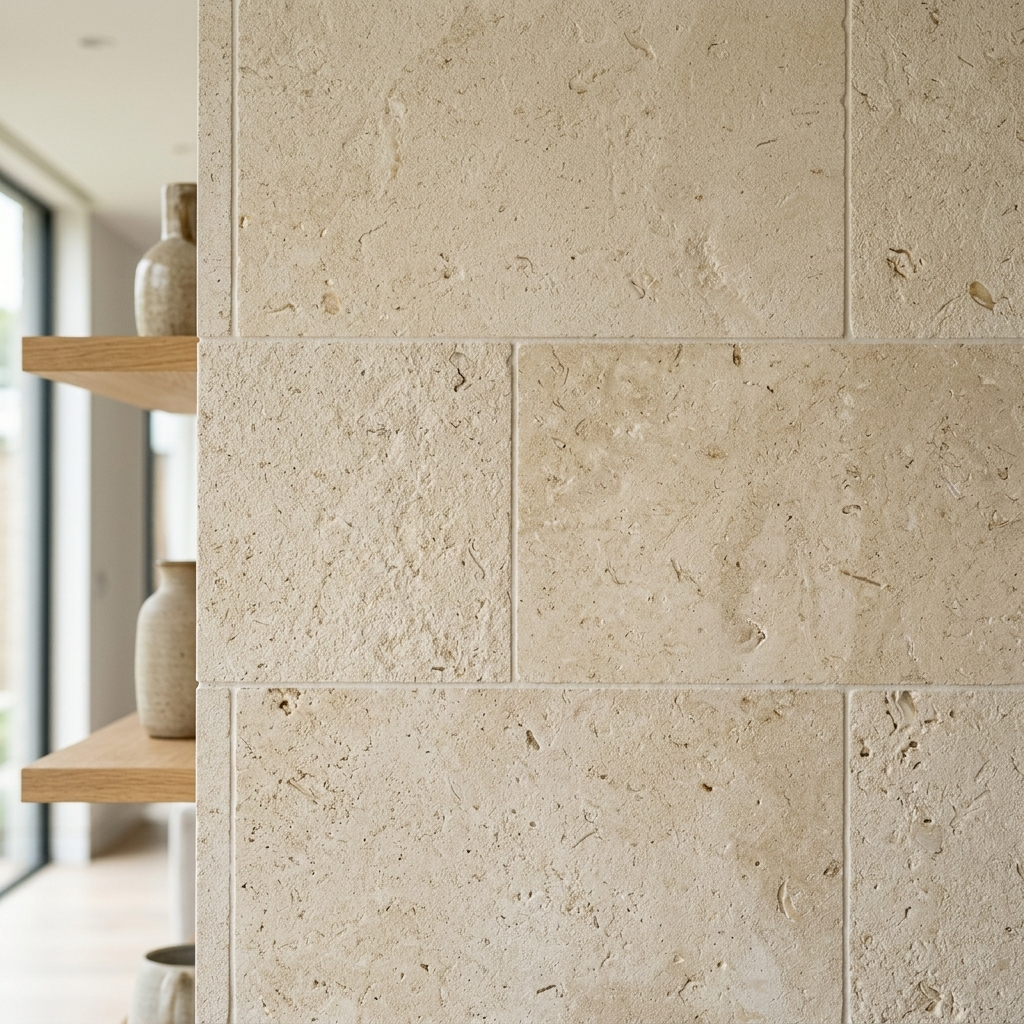
\includegraphics[width=0.7\linewidth]{images/figura_21.png}
    \caption{Aplacado de piedra caliza natural Crema de Antequera}
    \label{fig:aplacado}
\end{figure}


\subsection{Alféizares Cerámicos Naturales (Vierteaguas)}
\label{wall:alfeizar_cer}
\textbf{Descripción:} Piezas de alfeizar vierteaguas en gres extruido natural de alta resistencia, tipo klinker o similar, en color terracota/arcilla mate. Diseñados con goterón inferior y pendiente del 10 % para evitar filtraciones y manchas de escorrentía en el paramento pintado de la fachada. Suministrado por distribuidores locales de Sevilla. Ficha de producto disponible en el \href{https://www.obramat.es/}{Sitio Web} de Obramat.

\textbf{Uso en la memoria:} Vierteaguas y alféizares en las 4 ventanas exteriores (Ap. 3.1).

\begin{figure}[H]
    \centering
    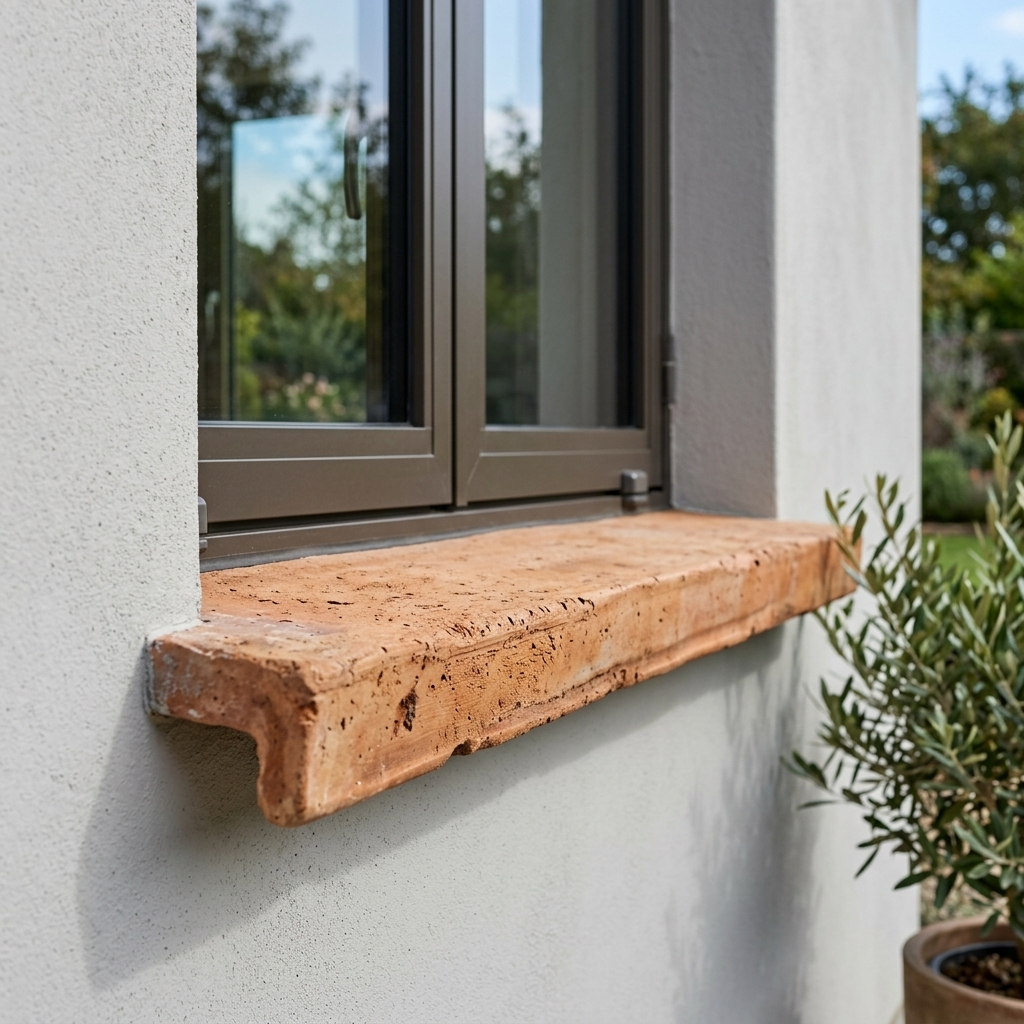
\includegraphics[width=0.7\linewidth]{images/figura_22.png}
    \caption{Vierteaguas de gres natural klinker terracota}
    \label{fig:alfeizar_cer}
\end{figure}


\subsection{Pinturas Interiores Ecológicas}
\label{wall:pintura_int}
\textbf{Descripción:} Pintura plástica mate al agua de alta cubrición y lavabilidad, modeloUno Cero Sin OlordePinturas Montó(libre de COVs, certificación A+ de emisiones), en colores Blanco Hueso (base general) y Arena Beige (paredes de acento). Disponible en Tiendas Montó de Sevilla. Ficha de producto disponible en el \href{https://www.pinturasmonto.com/es/productos/uno-cero-sin-olor}{Sitio Web de Pinturas Montó}.

\textbf{Uso en la memoria:} Pintado de paredes interiores en colores beige y blanco roto (Ap. 2.3).

\begin{figure}[H]
    \centering
    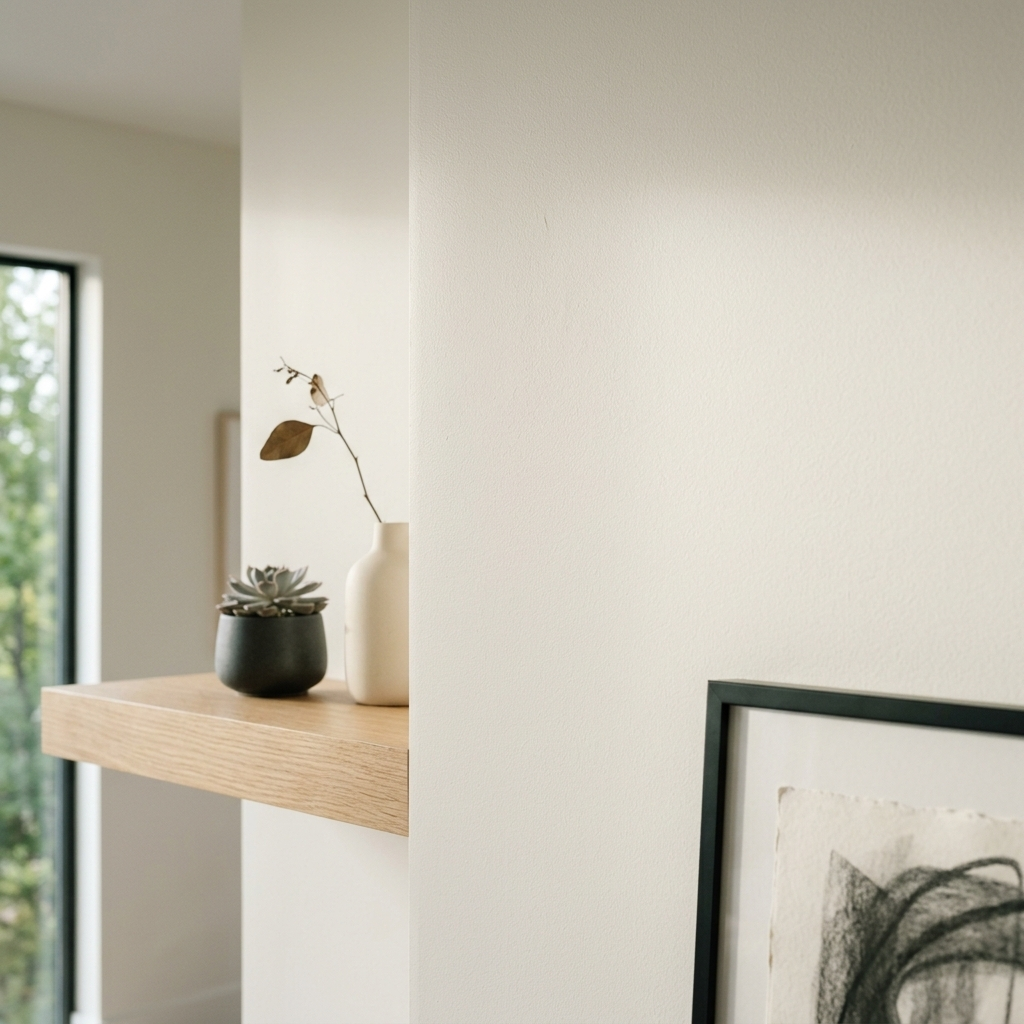
\includegraphics[width=0.7\linewidth]{images/figura_23.png}
    \caption{Pintura ecológica de interior Uno Cero Sin Olor}
    \label{fig:pintura_int}
\end{figure}


\subsection{Barras de Obra Paneladas y Encimeras}
\label{sec:cat_6_5}
\subsection{Estructura Base de Mampostería}
\label{bar:mamp}
\textbf{Descripción:} Tabiquería de fábrica realizada con ladrillo cerámico hueco doble (formato 7x12x25 cm) recibido con mortero de cemento de dosificación M-5 (1 parte de cemento CEM II/B-L 32.5 R por 4 partes de arena de río de la provincia de Sevilla). Acabado mediante enfoscado de cemento y enlucido de yeso en sus caras internas.

\textbf{Uso en la memoria:} Estructura de soporte de la barra de servicio interior (Ap. 2.2).


\subsection{Panelado Exterior de Cerámica Relieve}
\label{bar:relieve}
\textbf{Descripción:} Azulejo cerámico esmaltado de formato 7,5×30 cm con relieve estriado listonado vertical, gamaStripes Transition (oStripes Earth) del fabricante españolWow Design(o serieStrip SanddeEquipe Cerámicas), colocado en vertical con junta fina rectificada de 1 mm y rejuntado con mortero impermeable del mismo tono. Ficha de producto disponible en el \href{https://wowdesignspace.com/collection/stripes/}{Sitio Web} de WOW Design.

\textbf{Uso en la memoria:} Revestimiento frontal de la barra de servicio con relieve vertical (Ap. 2.2).

\begin{figure}[H]
    \centering
    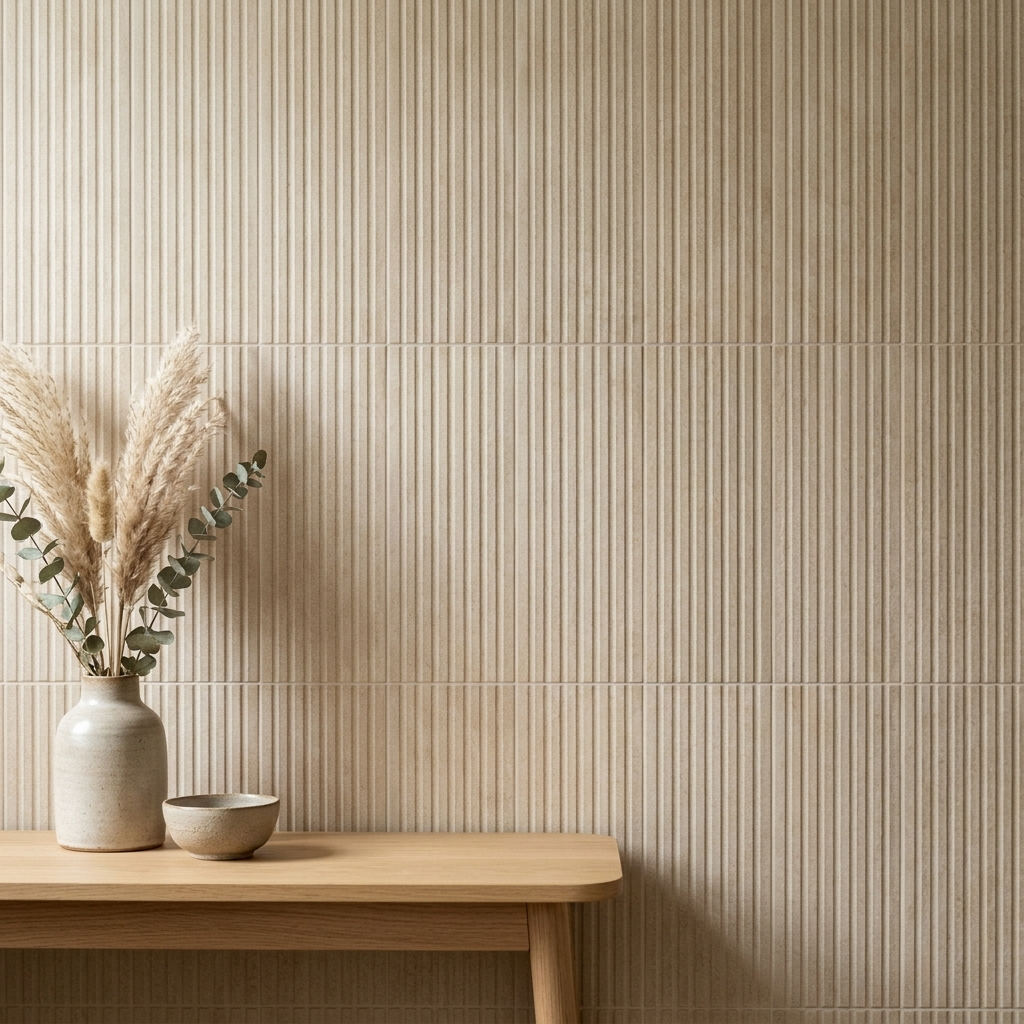
\includegraphics[width=0.7\linewidth]{images/figura_28.png}
    \caption{Azulejo cerámico estriado Stripes de WOW Design}
    \label{fig:relieve}
\end{figure}


\subsection{Encimera de Trabajo y Servicio}
\label{bar:krion}
\textbf{Descripción:} Superficie sólida mineral (Solid Surface) antibacteriana y autolimpiable de la firma españolaKrionde Porcelanosa (modelo Krion K-Life 1100 Snow White), de 12 mm de espesor, instalada con juntas químicas invisibles del mismo color. Ficha de producto disponible en el \href{https://www.krion.com/es/krion-solid-surface}{Sitio Web de Krion}.

\textbf{Uso en la memoria:} Coronación de encimera en barra de servicio interior (Ap. 2.2).

\begin{figure}[H]
    \centering
    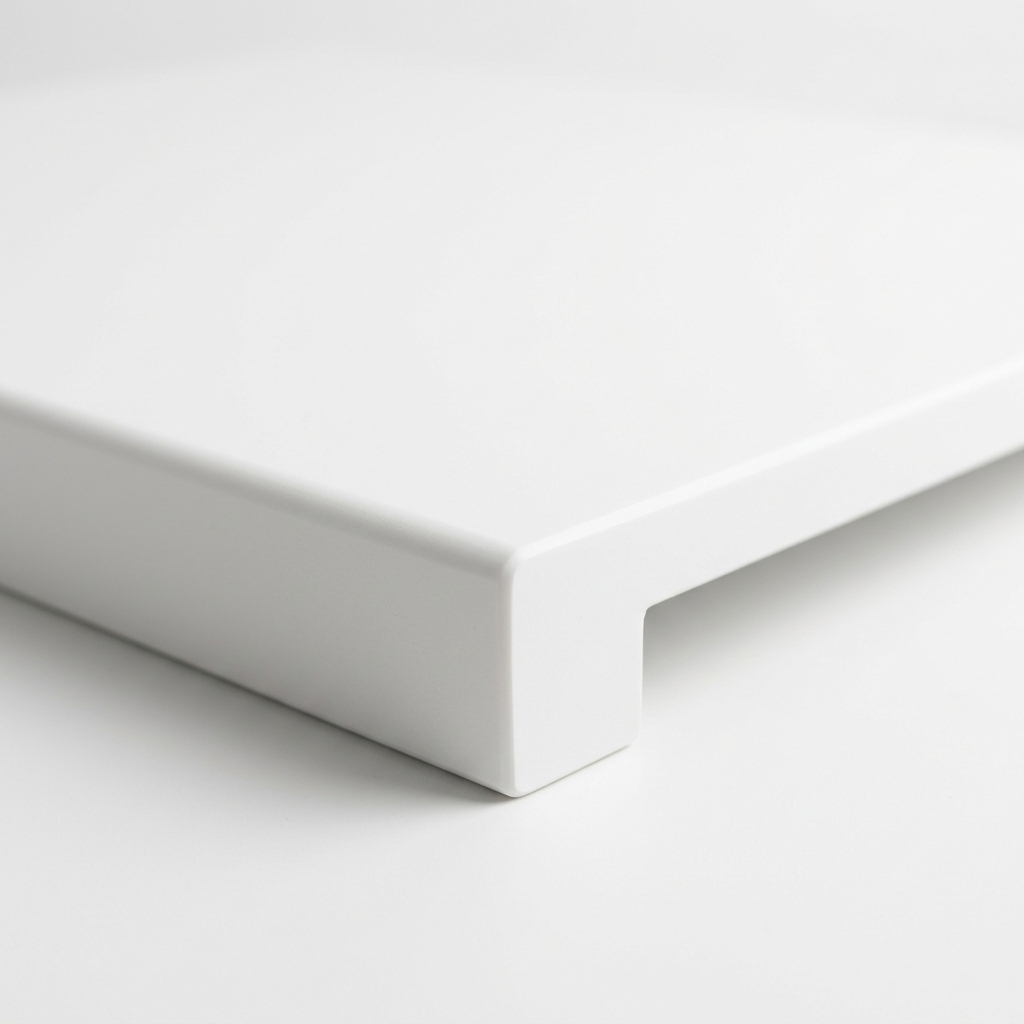
\includegraphics[width=0.7\linewidth]{images/figura_29.png}
    \caption{Encimera de Krion Solid Surface Snow White}
    \label{fig:krion}
\end{figure}


\subsection{Puertas, Carpinterías y Cerramientos de Acceso}
\label{sec:cat_6_6}
\subsection{Puerta de Acceso Principal (Millennium Plus 70)}
\label{door:acceso}
\textbf{Descripción:} Puerta batiente de doble hoja fabricada con perfiles de aluminio extruido con rotura de puente térmico (RPT) lacados en color negro mate (RAL 9005), con acristalamiento de seguridad doble (laminar 3+3.2 con cámara de aire para aislamiento térmico y acústico). Equipada con tiradores tubulares verticales de acero inoxidable lacados en negro mate, bisagras reforzadas de alta durabilidad y cerradura de seguridad. Suministrada e instalada por carpintería metálica local de Sevilla. Ficha de producto disponible en el \href{https://www.ventanasfraktal.es/ventanas/puertas-cortizo/millennium-plus-70/}{Sitio Web de Ventanas Fraktal}.

\textbf{Uso en la memoria:} Puertas peatonales de acceso principal en fachada exterior (2 uds.) (Ap. 3.2).

\begin{figure}[H]
    \centering
    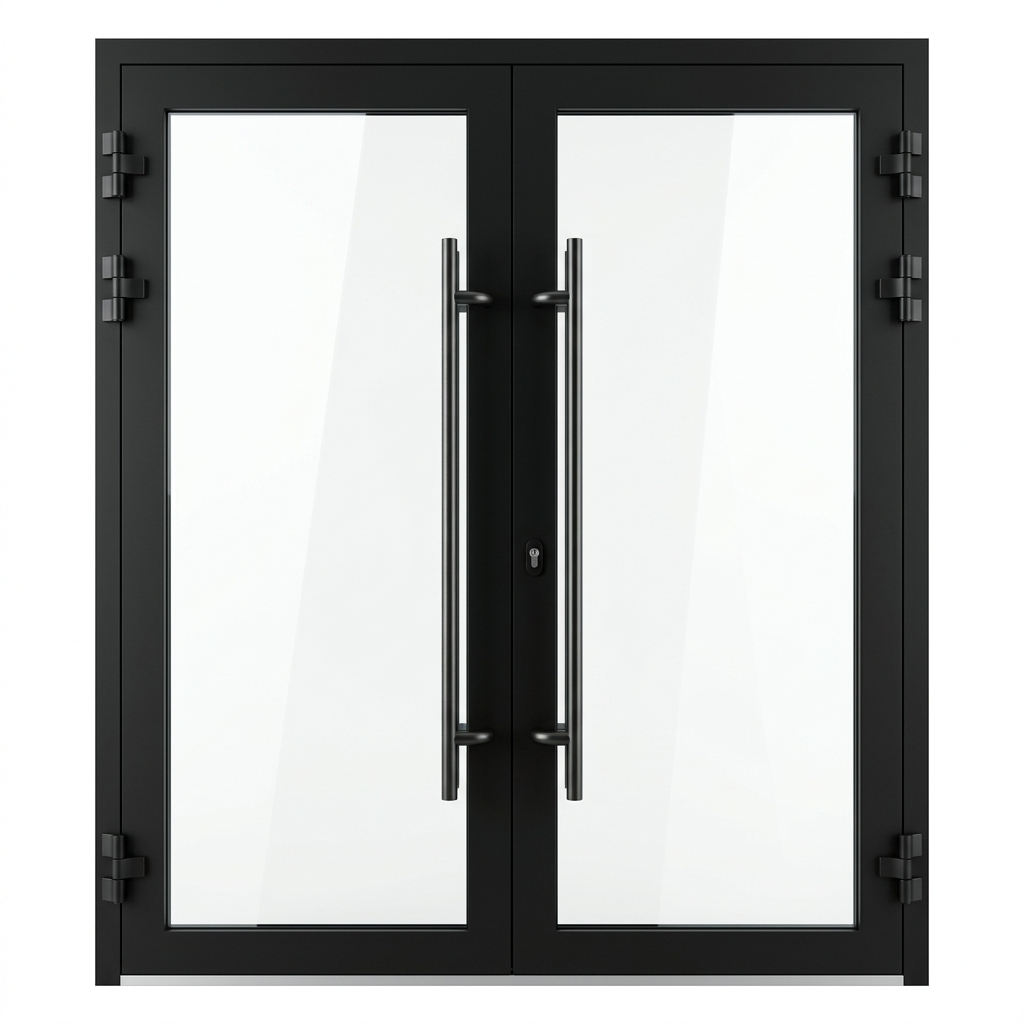
\includegraphics[width=0.7\linewidth]{images/figura_31.png}
    \caption{Puerta de aluminio peatonal Millennium Plus 70}
    \label{fig:acceso}
\end{figure}


\subsection{Carpintería de Ventanas (Aluminio Negro Mate)}
\label{door:ventana}
\textbf{Descripción:} Perfilería de aluminio practicable y oscilobatiente de la gama Cortizo (o similar) con rotura de puente térmico (RPT), lacada en color negro mate (RAL 9005) a juego con las carpinterías de la puerta principal. Doble acristalamiento de seguridad con cámara de aire deshidratada (tipo Climalit 4/16/4) para asegurar un óptimo aislamiento térmico y acústico en los comedores. Ficha de producto disponible en el \href{https://www.ventanasfraktal.es/ventanas/}{Sitio Web de Cortizo}.

\textbf{Uso en la memoria:} Ventanas exteriores (4 uds.) de la fachada de la cafetería del Hospital de Rehabilitación y Traumatología (Ap. 3.2).


\subsection{Pérgolas y Sistemas de Sombreamiento}
\label{sec:cat_6_7}
\subsection{Toldo Corredero / Palillero Plano}
\label{perg:toldo}
\textbf{Descripción:} Sistema de toldo plano de palillería corredero confeccionado a medida. Lona acrílica de alta densidad (300 g/m²) en color beige/arena, con alta protección UV y tratamiento repelente al agua y la suciedad. Estructura de perfiles de aluminio y guías superiores con rodamientos para un deslizamiento manual suave mediante cordón náutico de tracción y poleas. Diseñado para su instalación entre paredes o bajo estructura existente, garantizando una óptima protección solar. Ficha de producto disponible en el \href{https://www.cortinadecor.com/toldos/toldo-palillero}{Sitio Web de Cortinadecor}.

\textbf{Uso en la memoria:} Toldos correderos planos para protección solar en la fachada exterior (Ap. 3.1).

\begin{figure}[H]
    \centering
    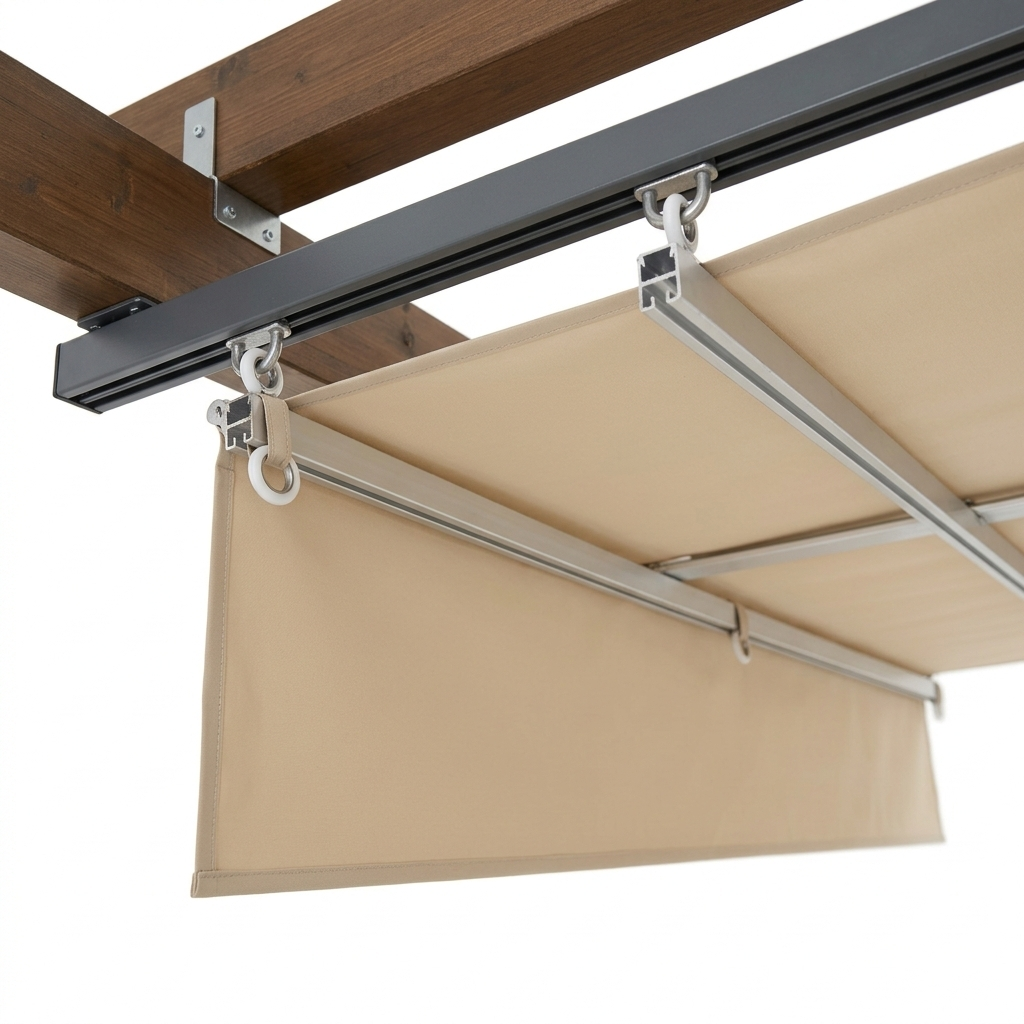
\includegraphics[width=0.7\linewidth]{images/figura_32.png}
    \caption{Toldo plano de palillería corredero}
    \label{fig:toldo}
\end{figure}


\subsection{Vegetación y Elementos de Paisajismo (Biofilia)}
\label{sec:cat_6_8}
\subsection{Maceteros de Exterior (Hormigón Gris)}
\label{veg:maceta_ext}
\textbf{Descripción:} Maceteros y jardineras de diseño contemporáneo fabricados en hormigón/cemento gris texturado mate, impermeabilizados en su interior y con drenaje adecuado. Incluye un modelo cúbico (50×50×50 cm) y un modelo de jardinera rectangular (100×40×40 cm). Disponibles en distribuidores locales en Sevilla.

\textbf{Uso en la memoria:} Planters de hormigón en la acera peatonal exterior (Ap. 3.4).


\subsection{Especies Vegetales de Exterior (Olivo y Arbustos)}
\label{veg:ext}
\textbf{Descripción:} Suministradas por vivero local (Viveros Sevillao similar en el Aljarafe) preparadas en contenedor de transporte y listas para trasplante: ˆOlea europaea (Olivo):Ejemplares de olivo ornamental joven de copa podada y tronco leñoso, adaptados a contenedor, que aportan naturalidad e identidad mediterránea. ˆVegetación Arbustiva de Base:Mezcla de plantas de exterior de porte bajo y hoja verde persistente para rellenar la base de la jardinera rectangular.

\textbf{Uso en la memoria:} Olivo ornamental y plantas arbustivas en los maceteros exteriores (Ap. 3.4).


\subsection{Maceteros de Interior (Gran Formato)}
\label{veg:maceta_int}
\textbf{Descripción:} Maceteros cilíndricos verticales de gran porte (altura 70 cm, diámetro 40 cm) en resina de polietileno lacada en blanco mate o ecru mate, equipados con doble pared y sistema de autorriego integrado. Adquiridos en distribuidores locales de jardinería técnica en Sevilla.

\textbf{Uso en la memoria:} Maceteros verticales de gran formato distribuidos en el interior (Ap. 2.3).


\subsection{Especies Vegetales de Interior (Gran Porte)}
\label{veg:int}
\textbf{Descripción:} ˆMonstera deliciosa (Costilla de Adán):Planta de interior trepadora de hoja grande y lobulada verde brillante, de 1.5 metros de altura. ˆFicus lyrata (Ficus de hoja lira):Arbusto ornamental de interior de tronco leñoso erecto y grandes hojas coriáceas en forma de lira, de 1.8 metros de altura.

\textbf{Uso en la memoria:} Plantas de Monstera deliciosa y Ficus lyrata en maceteros interiores (Ap. 2.3).


\subsection{Macetas de Mesa (Interior)}
\label{veg:maceta_mesa}
\textbf{Descripción:} Pequeños cuencos cerámicos o de cemento (10×10 cm) con mezcla de suculentas naturales (Echeveria,Sedum,Crassula) plantadas sobre sustrato de drenaje rápido. Suministrado por vivero local.

\textbf{Uso en la memoria:} Minimacetas con suculentas naturales dispuestas sobre las mesas de los comedores (Ap. 2.3).


\newpage



\end{document}
